\documentclass[11pt,letterpaper]{article}

%\usepackage{fontspec}
%\usepackage[utf8]{inputenc}
\usepackage{textcomp,marvosym}
\usepackage{amsmath,amssymb}
\usepackage[left]{lineno}
\usepackage{changepage}
\usepackage{rotating}
\usepackage{natbib}
\usepackage{setspace}
\usepackage{}
\usepackage{fancyhdr}
\usepackage{graphicx}
\doublespacing

\raggedright
\textwidth = 6.5 in
\textheight = 8.25 in
\oddsidemargin = 0.0 in
\evensidemargin = 0.0 in
\topmargin = 0.0 in
\headheight = 0.0 in
\headsep = 0.5 in
\parskip = 0.1 in
\parindent = 0.1in

% Bold the 'Figure #' in the caption and separate it from the title/caption with a period
% Captions will be left justified
\usepackage[aboveskip=1pt,labelfont=bf,labelsep=period,justification=raggedright,singlelinecheck=off]{caption}

% Remove brackets from numbering in List of References
%\makeatletter
%\renewcommand{\@biblabel}[1]{\quad#1.}
%\makeatother

\pagestyle{myheadings}
\pagestyle{fancy}
\fancyhf{}
\lhead{Fairchild et al., submitted to GEOLOGY}
\rhead{\thepage}

\begin{document}

\begin{flushleft}
{\Large \textbf{A matter of minutes: Breccia dike paleomagnetism provides evidence for rapid crater modification}}
\\
Luke M. Fairchild\textsuperscript{1,2},
Nicholas L. Swanson-Hysell\textsuperscript{1},
Sonia M. Tikoo\textsuperscript{1,3}
\\
\bigskip
\textsuperscript{1} Department of Earth and Planetary Science, University of California, Berkeley, CA, USA
\\
\textsuperscript{2} Department of Geology, Carleton College, Northfield, Minnesota, USA
\\
\textsuperscript{3} Berkeley Geochronology Center, 2455 Ridge Road, Berkeley, CA 94709, USA
\bigskip

\end{flushleft}

\noindent\textit{This article has been submitted for consideration at GEOLOGY (published by the Geological Society of America).}

\linenumbers

\section*{ABSTRACT}
Following an impact event, a crater's transient structure adjusts gravitationally. Within complex craters, a central uplift rises and collapses resulting in large-scale rotations of the target rock. Estimated crater modification rates from numerical models indicate that complex impact craters likely modify to a structurally stable state within tens of seconds to several minutes after initial excavation. However, there is little direct geologic evidence constraining these rates. We show how paleomagnetic measurements of clastic breccia dikes emplaced during crater excavation can be used to constrain the rate of crater modification within the central uplift of the $\sim$34 km diameter Slate Islands impact structure, Ontario, Canada. The uniformity and linearity of paleomagnetic directions among the clasts and matrix of breccia dikes throughout the impact structure indicate that breccia dikes were frictionally heated above the magnetite Curie temperature (580\textdegree C) during their emplacement and subsequently cooled \textit{in situ} through magnetic blocking temperatures. The tight grouping of these paleomagnetic directions implies that these breccia dikes cooled and locked in magnetic remanence over a time interval in which the impact structure was not experiencing structural rotations and had already reached a stable state. Conductive cooling of the thinnest sampled breccia dike would have led to the recording of magnetic remanence approximately six minutes after emplacement. This constraint necessitates a stable crater structure only minutes after impact and presents a rare case in which a geological process can be resolved on such a short timescale.


\section*{INTRODUCTION}
Breccia dikes are a ubiquitous feature of impact craters that can be broadly characterized as injections of fragmented or molten target rock into the crater subsurface during an impact event. These dikes can be categorized by their matrix composition as either: 1) impact melt glass dominated (Type A of \cite{Lambert1981a}) or 2) clastic (Type B of \cite{Lambert1981a}). Type A breccia dikes (also commonly referred to as pseudotachylites) are emplaced during shock compression, whereas thicker, Type B clastic breccia dikes are emplaced immediately after the passage of the shock wave, during dilatation of the target rock and excavation of the transient crater \citep{Lambert1981a, Masaitis2005a}.

The Slate Islands archipelago in northern Lake Superior exposes portions of the eroded central uplift of an otherwise underwater crater approximately 34 km in diameter. Clastic breccia dikes within the Slate Islands are abundant and well-exposed \citep{Dressler1997a}. These dikes have irregular branching geometries with individual branches ranging from cm-scale to several meters in thickness (Fig. \ref{fig:photo}). The breccia clasts are generally polymictic and sourced from the variety of target rocks through which the dike intruded, possibly at cumulative distances $>$2 km \citep{Dressler1997a}. However, clast lithologies are dominated by that of the immediately surrounding host rock. Clasts are angular to sub-angular and range from sub-millimeter to more than 3 meters in diameter (Fig. \ref{fig:photo}). The matrix comprises target rock detritus composed of monomineralic grains and lithic fragments and is either green or red in color (Fig. \ref{fig:photo}).

\begin{figure}
\noindent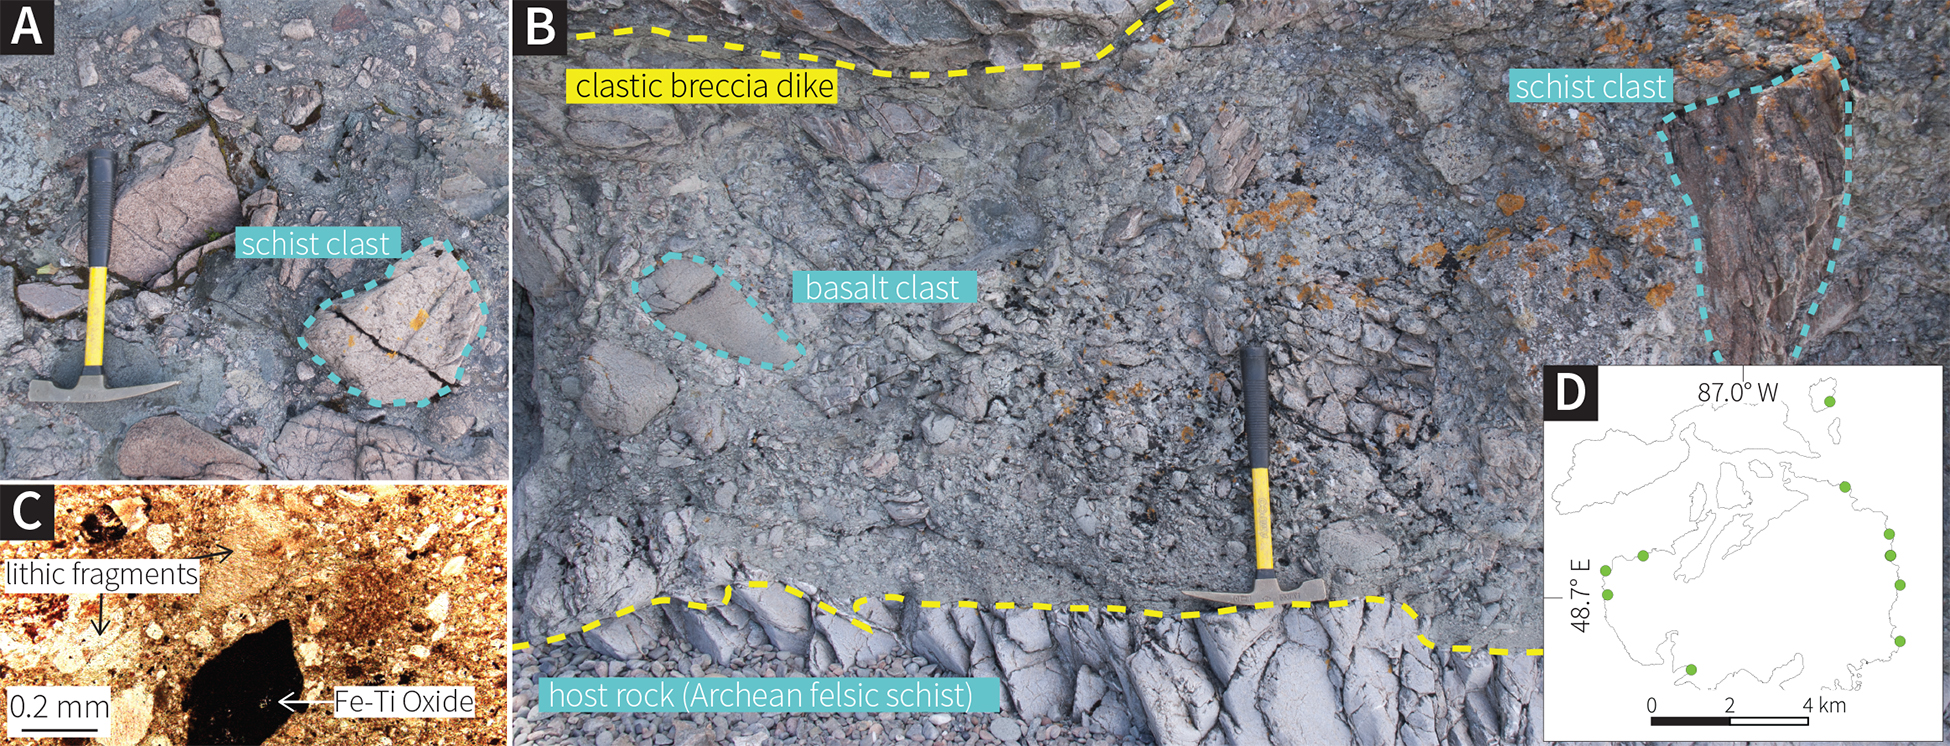
\includegraphics[width=\textwidth]{figures/Breccia_Dike_Photos.jpg}

\caption{\footnotesize{\textbf{Outcrop photos of breccia dike PI24 (a, b) and photomicrograph (plane polarized light) of breccia dike PI15. The inset map of the Slate Islands (d) shows the location of studied breccia dikes.}}}
\label{fig:photo}
\end{figure}


Previous paleomagnetic analysis of clastic breccia dikes in the Slate Islands found that samples of the dike matrix record a unidirectional magnetization with the same direction as a partial overprint recorded by unbrecciated host rocks \citep*{Halls1979a}. Breccia dike clasts were not sampled in the \cite{Halls1979a} study. Two plausible origins of this matrix magnetization include: 1) thermoremanent magnetization (TRM) acquired by frictional heating during the breccia dike's emplacement (as interpreted by \cite{Halls1979a}) and 2) chemical magnetization (CRM) imparted by the precipitation of new ferromagnetic minerals during post-impact hydrothermal activity. The paleomagnetism of breccia dike clasts provides a way to discriminate between the thermal and chemical hypotheses. Due to their lower permeability than the matrix, breccia clasts are less susceptible to chemical remagnetization. If the remanence held by the matrix is a CRM, the interior of many clasts would be relatively unaffected and retain pre-impact remanence directions. However, if the dikes were heated above ferromagnetic Curie temperatures during emplacement, the clasts should be fully remagnetizated in contrast to the partial overprints observed within unbrecciated host rock \citep{Halls1979a}. If the breccia dike magnetizations were thermally acquired during their emplacement, the remanence directions would have been locked in quickly within thin dikes and could have subsequently rotated if crater modification was ongoing over a prolonged period. In this way, the magnetization of breccia dikes could provide useful constraints on the timeline of crater modification.

\section*{METHODS and RESULTS}

To evaluate the consistency of breccia dike paleomagnetic directions, and to establish whether breccia clasts were fully overprinted in addition to the matrix, we collected samples for paleomagnetic analysis from 11 breccia dike sites throughout the impact structure, five of which were amenable to the sampling of clasts. In the UC Berkeley Paleomagnetism Laboratory, samples were thermally demagnetized at increments of 25\textdegree C or less up to a peak temperature of 580\textdegree C (the Curie temperature of magnetite). For two sites (DeI2 and PI2), heating to the 680\textdegree C N\'eel temperature of hematite was required for complete demagnetization. Small present local field overprints were removed by heating to $\sim$200\textdegree C (Fig. \ref{fig:pmag}). Consistent with the work of \cite{Halls1979a}, matrix samples of dikes throughout the impact structure yield magnetization components that persist to 580\textdegree C and conform to a single direction. Likewise, the remanence directions of clasts from the dikes are unidirectional up to 580\textdegree C and yield the same direction as the matrix (Fig. \ref{fig:pmag}b). Paleomagnetic conglomerate tests \citep{Watson1956a} conducted on these clast magnetization directions held by magnetite show that directional randomness can be rejected at the 99$\%$ confidence level for all 5 breccia dikes in which clasts were sampled.\footnote{GSA Data Repository item 2016XXX, paleomagnetic data and statistical test results, and details of the conductive cooling model, is available online at www.geosociety.org/pubs/ft2016.htm, or on request from editing@geosociety.org or Documents Secretary, GSA, P.O. Box 9140, Boulder, CO 80301, USA.} This behavior is seen both for clasts of Mesoproterozoic diabase/basalt and Archean metamorphics and the thermal unblocking spectra are consistent with (titano)magnetite. This result is a strong indicator that the clasts were thermally remagnetized after their emplacement. In addition to the remanence held by magnetite, 2 dikes with a red appearance (the majority of sampled dikes have a green-colored matrix) in the field also have remanence in the matrix held by hematite that is removed at higher unblocking temperatures following removal of a distinct magnetite component. These magnetizations held by hematite generally correspond to the impact direction as well and were likely acquired during either post-impact cooling or hydrothermal activity.

\begin{figure}
\noindent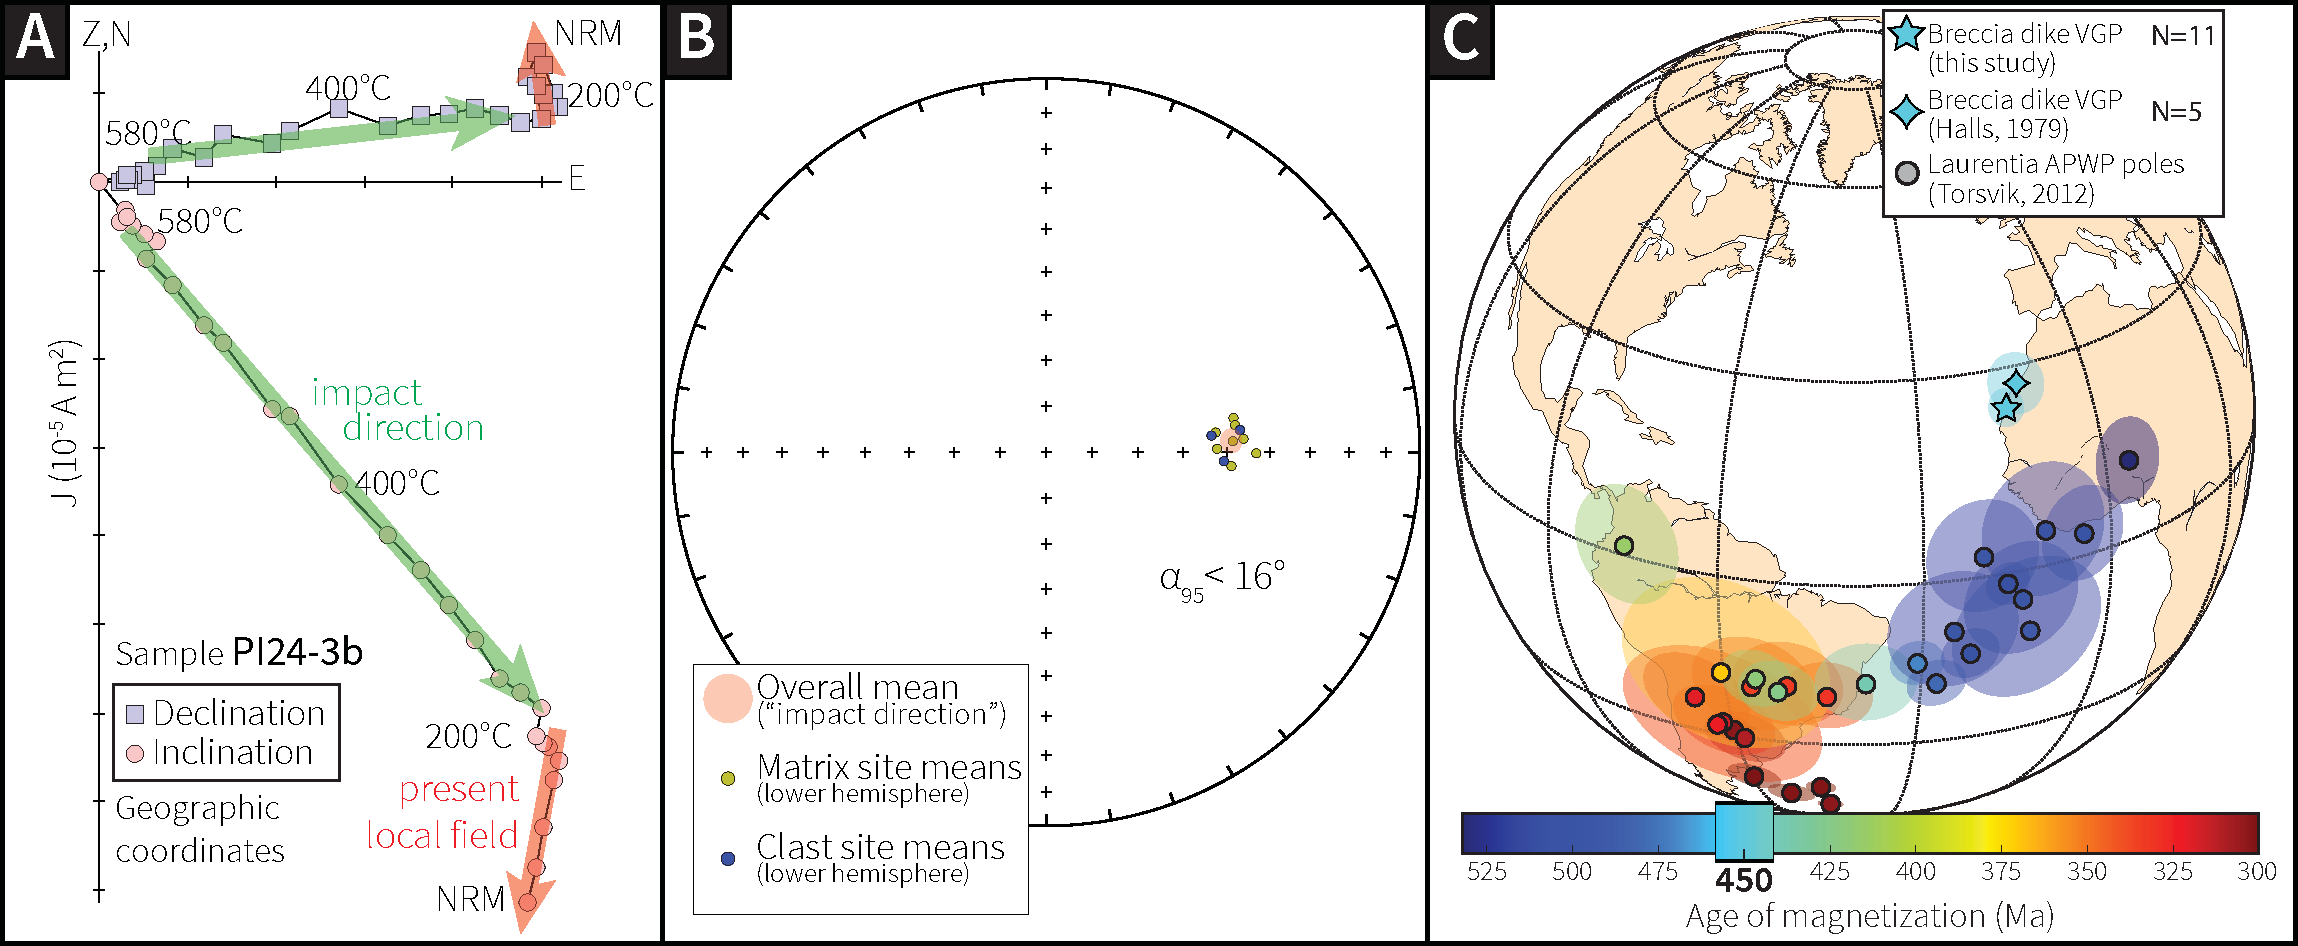
\includegraphics[width=\textwidth]{figures/Pmag_data.pdf}
\caption{\textbf{\footnotesize{Paleomagnetic data of Slate Islands clastic breccia dikes. a) Example Zijderveld plot of paleomagnetic data from a breccia clast sample, with least squares fits indicated by labeled arrows. b) Equal area plot with site means from both matrix and clast samples and their overall mean with associated $\alpha_{95}$ confidence ellipse. c) Comparison of Slate Islands VGP (this study; \citet{Halls1979a}) with the Paleozoic APWP of Laurentia \citep{Torsvik2012a}.}}}
\label{fig:pmag}
\end{figure}

In contrast to the clasts of breccia dikes, host rocks throughout the crater retain pre-impact magnetizations with partial impact overprints \citep{Halls1979a}. These pre-impact directions are particularly coherent and well-resolved in Keweenawan lava flows exposed on the west side of Patterson Island. In these flows, impact related overprints are typically removed by $\sim$275\textdegree C. However, a flow hosting an impact breccia dike reveals an overprint persisting to higher temperatures. We interpret this result as a positive baked contact test consistent with local heating associated with breccia dike emplacement (see \textit{Breccia dike host rock} section of the Data Repository). We observed similar behavior in Archean schist host rock. For example, at site PI16, the same metamorphic lithology which is fully overprinted to unblocking temperatures $>$500\textdegree C when encountered as breccia clasts has remanence unrelated to the impact direction removed at high temperatures in samples collected multiple dike widths away. The partial overprinting of host rock demonstrates that the full overprinting of breccia clasts is the result of localized heating that reached significantly higher temperatures than the more widespread heating of central uplift target rocks.

\section*{DISCUSSION}

\subsection*{Direction of impact magnetization}
The magnetization of breccia dikes and the overprint in Slate Islands host rocks record the local geomagnetic field at the time of the Slate Islands impact. In contrast, similar lithologies as some overprinted target rocks found outside the crater are minimally overprinted with stable primary magnetizations that date to their formation in the 1.1 Ga Midcontinent Rift \citep{Halls1975a, Swanson-Hysell2014b}, supporting the interpretation that the overprint is indeed associated with the impact event rather than being associated with broader tectonic processes.  As described by \cite{Halls1979a}, the virtual geomagnetic pole (VGP) calculated from breccia dike paleomagnetic directions corresponds to Laurentia's apparent polar wander path (APWP) at ca. 1000 Ma (the ``Grenville Loop"). This age assignment is consistent with geological constraints that require that the impact occurred after cessation of Midcontinent Rift magmatism (ca. 1085 Ma). \cite{Dressler1999a} interpreted a plateau in the $^{40}$Ar-$^{39}$Ar release spectrum of a single pseudotachylite sample as implying a Silurian age for the impact crater. The integrated age derived from this spectrum was 436 $\pm$ 3 Ma. Two Midcontinent Rift basalt samples from the Slate Islands crater were dated by the same study and yielded integrated ages of ca. 1074 and ca. 990 Ma; discordance in the low temperature portion of the $^{39}$Ar release spectra are consistent with a more recent heating event.

The breccia dike VGP is $\sim$47\textdegree\ from the Silurian paleopoles of the Laurentia APWP and $\sim$35\textdegree\ from the Ordovician paleopoles (\cite{Torsvik2012a}; Fig. \ref{fig:pmag}c). Given that the magnetization of the breccia dikes would have been quickly acquired during cooling, the calculated pole is not time-averaged and should not be expected to fall directly on the APWP. However, even with this lack of time-averaging, a 50\textdegree\ difference from the APWP is quite large and calls the Silurian age into question. If the impact did occur in the Silurian, the crater likely formed during a period of significant geomagnetic deviation from the geographic pole (i.e. an excursion). The geocentric axial dipole (GAD) model TK03.GAD gives a $\sim$6\% probability for $>$30\textdegree~divergence of a VGP from geographic north and $\sim$3\% probability for $>$40\textdegree~divergence \citep{Tauxe2004a} making such a deviation a plausible, but low probability, event.

\subsection*{Timescale of crater modification}

Numerical models of large impacts have provided understanding of a process that is too rare to be directly observed on human time scales \citep{Pierazzo2004a}. These hydrocode models indicate that the main stages of impact cratering (compression, excavation, and modification; \cite{Gault1968a}) are rapid and occur on second to minute timescales. For example, hydrocode simulations of a $\sim$40 km terrestrial impact crater (similar in size to the Slate Islands impact structure) showed that crater modification was largely complete $\sim$300 s ($\sim$5 minutes) after the impact \citep{Collins2014a}. However, \cite{Melosh1999a} noted that the material behaviors assumed in hydrocode models are often insufficient descriptors of the dynamic rock failure that occurs during crater modification. While it remains unclear how significantly the duration of crater modification would deviate from the estimates of these models, it is apparent that additional geophysical and observational constraints are valuable for understanding the timing of this process.

One such constraint comes from the melt sheets of the Boltysh and Manicouagan impact structures which have been observed to encircle the central uplifts, implying that the melt pool solidified after central uplift formation \citep{Melosh1999a}. From this observation, \cite{Melosh1999a} estimated the duration of central uplift formation to be $<$100 seconds, the calculated timeframe for viscosity increase of the melt associated with melt-clast heat exchange \citep{Onorato1978a}. However, given that complete solidification of the Manicouagan melt is estimated to have taken ca. 35 years at 10 meters from the edge and ca. 1600 years 100 meters into the melt \citep{Onorato1978a}, evidence of melt sheet deformation by the central uplift might not be preserved due to prolonged convection within the melt pool.

The complete overprinting of magnetite-held clast magnetizations, in contrast to the partial overprints of the same lithologies in host rocks, strongly support the hypothesis that clastic breccia dikes in the Slate Islands were frictionally heated above 580\textdegree C and acquired a full TRM. Because of their thermal origin, the magnetic directions of clastic breccia dikes serve as effective structural tracers for segmented blocks of the impact structure: as breccia bodies cool through magnetic blocking temperatures, their paleomagnetic directions would record any relative rotations of their host rock during crater modification. If their cooling rates can be constrained, these impact features may thereby provide a relative timeline of crater modification in the Slate Islands, with chaotic paleomagnetic directions among breccia dikes linked to structural rotations and, conversely, the alignment of these directions signaling a stable crater structure.

\begin{figure}
\noindent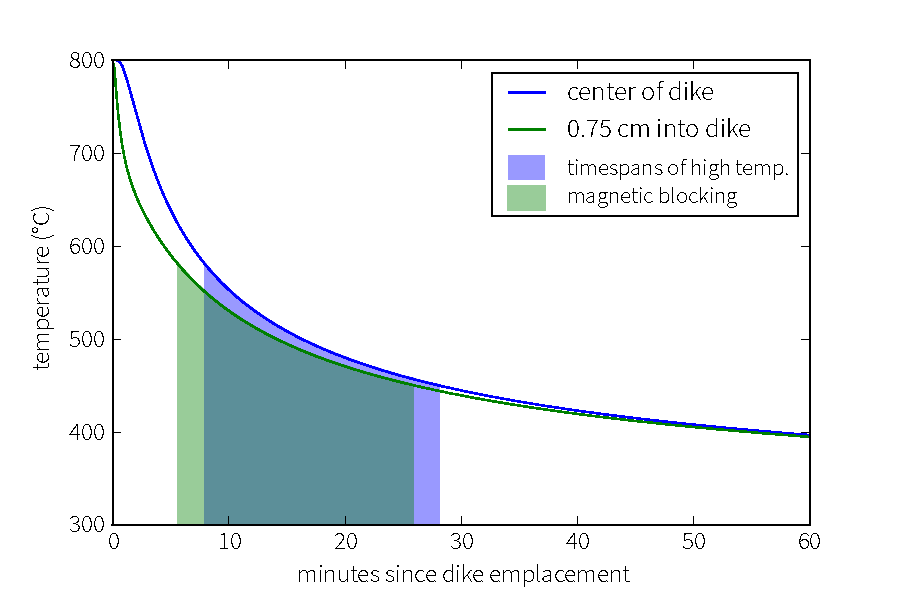
\includegraphics[width=0.65\textwidth]{figures/Cooling.pdf}
\caption{\textbf{\footnotesize{Conductive cooling model for a 4 cm-thick breccia dike emplaced at 800\textdegree C into host rock with a temperature of 275\textdegree C. The two curves represent the thermal history of the samples as the 2.5 cm diameter cores span from $\sim$0.75 cm to 2 cm from the dike edge. This model indicates that magnetic remanence began being blocked $\sim$6 minutes after dike emplacement--minimal rotation of the dike could have occurred from this time onwards given the unidirectional magnetization consistent with breccia directions across the crater.}}}
\label{fig:cooling}
\end{figure}

The linearity and directional uniformity of paleomagnetic data from breccia dikes across the impact structure suggest that the broader crater structure was stable throughout the timeline of breccia dike cooling and TRM acquisition. To quantify this timeline, it is necessary to assign a maximum emplacement temperature from which breccia dikes may have cooled. Petrographic analysis reveals an absence of autochthonous melt within the matrix of clastic breccia dikes (Fig. \ref{fig:photo}). Given the preponderance of uplifted Archean basement rock in the Slate Islands (schistose Archean metavolcanics and metaintrusives) and this lithology's dominant presence in clastic breccia dikes, we take this petrographic observation as a strong indicator that breccia dike emplacement temperatures did not exceed a schist solidus of $\sim$800\textdegree C \citep{Douce1998a, Whittington2009a}. A frictionally heated breccia dike would have undergone conductive cooling following emplacement. We take the simplest whole time solution of \cite{Delaney1987a} utilizing transient heat conduction theory for a plane of motionless material undergoing heat transfer to surrounding rock with no chemical reactions as a good representation of the problem. Conductive cooling of the thinnest sampled breccia dike (4 cm) from 800\textdegree C to estimated ambient temperatures of 275\textdegree C would have led to the recording of magnetic remanence (beginning upon cooling to 580\textdegree C) approximately 6 minutes after its emplacement (Fig. \ref{fig:cooling}; code in the Data Repository). Since emplacement of these clastic breccia dikes are understood to occur during the excavation stage of cratering prior to crater modification \citep{Lambert1981a, Masaitis2005a}, this 6 minute timespan represents the maximum duration of crater modification  that brought the Slate Islands central uplift to the gravitationally stable state recorded in breccia dike magnetizations.

\subsection*{ACKNOWLEDGEMENTS}
\footnotesize

This research was supported by the National Science Foundation through grants EAR-1316395 and EAR-1316375. Additional support to L.F. came from Class of '63 and Kolenkow-Reitz Fellowships awarded by Carleton College. Fieldwork in the Slate Islands was possible through research permits from Ontario Parks which are gratefully acknowledged.

\singlespacing

\newpage

\bibliographystyle{gsabull}
\bibliography{../../references/allrefs}

\end{document}
